\subsection{A derivation and implementation of an NS solver to simulate the two-dimensional cylinder wake flow.}

I implemented the initial finite-element Navier-Stokes (NS) solver \cite{Batchelor2000} to simulate two-dimensional cylinder wake flow -- the focus of which was on incompressible, viscous fluid flow \cite{Pope2000}. The inclusion of viscosity in the model and the application of no-slip boundary conditions \cite{White2006} is required to capture the nuanced behavior of real fluid flows often found in engineering applications. The presence of a square obstacle in the flow field allows us to investigate complex phenomena like separation, and vortex-shedding and wake formation \cite{Zdravkovich1997,Anderson1995}.

\subsubsection{Navier-Stokes Equations}
The NS equations, governing the fluid flow, are expressed as:
\begin{align}
    \frac{\partial u}{\partial t} + u \frac{\partial u}{\partial x} + v \frac{\partial u}{\partial y} &= -\frac{1}{\rho} \frac{\partial p}{\partial x} + \nu \left( \frac{\partial^2 u}{\partial x^2} + \frac{\partial^2 u}{\partial y^2} \right), \\
    \frac{\partial v}{\partial t} + u \frac{\partial v}{\partial x} + v \frac{\partial v}{\partial y} &= -\frac{1}{\rho} \frac{\partial p}{\partial y} + \nu \left( \frac{\partial^2 v}{\partial x^2} + \frac{\partial^2 v}{\partial y^2} \right), \\
    \frac{\partial u}{\partial x} + \frac{\partial v}{\partial y} &= 0,
\end{align}
where \( u \) and \( v \) are the fluid velocities in the x and y directions, respectively, \( p \) is the pressure, \( \rho \) is the fluid density, and \( \nu \) is the kinematic viscosity.

\subsubsection{Implementation}
The solver was implemented in Python, utilizing NumPy for efficient array computations. It initializes the velocity and pressure fields, and defines a cylinder obstruction in the flow. The update functions for velocity and pressure discretize the NS equations using finite difference methods. The solver handles complex phenomena like vortex shedding, illustrated in the simulations around the cylinder. Regular plotting intervals offer visual insights into the evolving fluid dynamics.

\subsubsection{Equations for Velocity and Pressure Update}
The velocity and pressure updates incorporate advection, pressure gradients, and diffusion:
\begin{align}
    u_{next} &= u - u \cdot dt \cdot \frac{\partial u}{\partial x} - v \cdot dt \cdot \frac{\partial u}{\partial y} - \frac{dt}{\rho} \frac{\partial p}{\partial x} + \nu \cdot dt \left( \frac{\partial^2 u}{\partial x^2} + \frac{\partial^2 u}{\partial y^2} \right), \\
    v_{next} &= v - u \cdot dt \cdot \frac{\partial v}{\partial x} - v \cdot dt \cdot \frac{\partial v}{\partial y} - \frac{dt}{\rho} \frac{\partial p}{\partial y} + \nu \cdot dt \left( \frac{\partial^2 v}{\partial x^2} + \frac{\partial^2 v}{\partial y^2} \right).
\end{align}

The pressure update, derived from the Poisson equation to ensure incompressibility, is given by:

\begin{equation}
\begin{split}
    p_{next} = \frac{1}{2 \cdot (dx^2 + dy^2)} \bigg(& (p_{i+1, j} + p_{i-1, j}) \cdot dy^2 \\
    & + (p_{i, j+1} + p_{i, j-1}) \cdot dx^2 \\
    & - \rho \cdot \left((u_{i+1, j} - u_{i-1, j}) / (2 \cdot dx) + (v_{i, j+1} - v_{i, j-1}) / (2 \cdot dy)\right)^2 \cdot dx^2 \cdot dy^2 \bigg).
\end{split}
\end{equation}

The simulation begins by initializing the velocity fields (representing fluid velocity in the x and y directions) and the pressure field. These initial conditions set the starting state of the fluid flow. The solver then discretizes the Navier-Stokes equations, which govern fluid motion, using finite difference methods in both time and space. To evolve the fluid dynamics over time, the solver employs update equations for velocity and pressure. 

\subsection{Unit testing}
A comprehensive suite of unit tests has been implemented to ensure the robustness and reliability of the code. These tests encompass various aspects of the project, including the functionality of classes and methods, and the integrity of the environment setup. The testing approach was mainly implemented to test the reliability of each step in the solution process. The tests were designed to leverage the modular structure of the solver, enabling the examination of various functional components and critical variables within each of the utilized solver files. Consequently, a multitude of unit tests were developed to confirm the correct functioning of these distinct code segments.
\\

Another key test is to ensure the Classes are properly initialized with default values. This test is vital for confirming that the simulation environment is set up correctly before any specific conditions or changes are applied. Additionally, we have also added tests targeted towards validating the internal mechanics of the Environment class, particularly ensuring that the methods responsible for updating matrices are functioning as expected. This is essential for the accuracy and reliability of the simulation's core computational algorithms. 
\\

These tests emphasize the importance of both verification and validation in software development. Verification ensures that the code meets set requirements and functions correctly, while validation confirms that these requirements make sense and serve the intended purpose. The tests implemented here serve as a testament to these principles, ensuring that the code not only works correctly but also fulfills its intended role effectively.
\\

In line with the overarching principles of testing, the tests are designed to be adversarial, aiming to rigorously challenge and scrutinize the code rather than simply confirming its functionality. This approach ensures that any potential defects are identified and addressed, thereby enhancing the reliability and robustness of the code. The tests also serve as documentation, explicitly stating the expectations and requirements of the code, and they play a crucial role in growing confidence in its reliability among users.

\subsection{Speed and efficiency}

I integrated Python's cProfile \cite{cprofile} module as a step in identifying performance bottlenecks and speed of runs.
This also allows for a concise comparison of the speed of the finite element NS solver against the PINN approximation. cProfile provides a detailed report on call frequency and duration of the code, which were pivotal in analyzing the efficiency. This integration was a key part of the process, allowing me to gather comprehensive performance data.
\\

Subsequently, I executed the simulation with cProfile enabled, capturing essential performance metrics. This was critical in understanding how different segments of my code impacted the overall runtime, providing a clear overview of the simulation's performance landscape. For the analysis of the profiling data, I utilized SnakeViz \cite{snakeviz}, a sophisticated graphical viewer designed for Python profiling data. This analysis was integral in visualizing and decoding performance bottlenecks, highlighting areas where optimization was necessary (Fig. \ref{fig:snake}). The benefits of this process were multifaceted. Firstly, profiling pinpointed specific functions or methods that consumed substantial time, guiding me towards target areas for optimization. Moreover, it facilitated efficient allocation of computational resources by illuminating the most resource-intensive parts of the code, thereby aiding in more informed decisions regarding optimization.
\\

\begin{wrapfigure}{r}{0.45\textwidth}
    \centering
    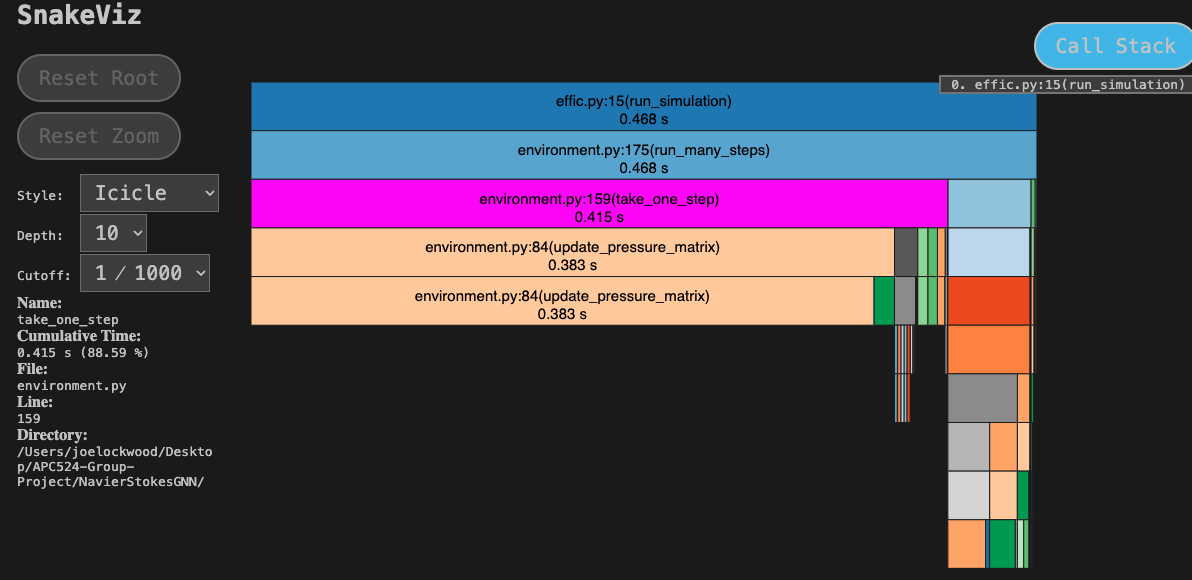
\includegraphics[width=0.45\textwidth]{Figures/final_report/Snake_prof.png}
    \caption{Sophisticated graphical viewer designed for Python profiling data using SnakeViz.}
    \label{fig:snake}
\end{wrapfigure}

With these insights, I embarked on optimizing and refining the code. By adjusting algorithms and refactoring, I was able to significantly improve the application’s performance. This process not only enhanced the efficiency of the code but also its quality and scalability, elevating the overall standard of the software. Additionally, these optimizations led to time and cost efficiencies, particularly beneficial in environments where computational resources are charged. The data-driven approach provided by profiling enabled me to make informed decisions, concentrating my efforts on modifications that offered substantial performance improvements.